	\subsection{Adapted Taxonomy of Virtualization Technology in On-Demand Grid Provisioning by \textit{Abdulhamid}}
	
	\begin{figure}[H]
		\centering
		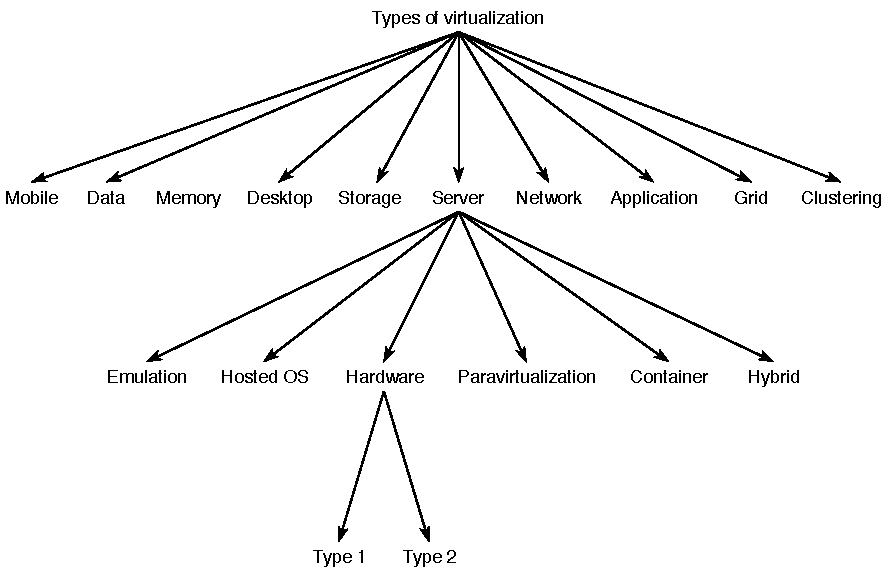
\includegraphics[width=9cm]{images/AmeenAndHamo2003.pdf}
		\vspace{-0.2cm}
		\caption{Taxonomy of virtualization by \textit{Radhwan Y. Ameen and Asmaa Y. Hamo} in 2013\footnotemark[200]{}.}
		\label{fig:TaxonomyOfVirtualizationBugnion}
	\end{figure}
	
	\footnotetext [200] {Figure bases on the study \textit{A Survey of Server Virtualization} by Radhwan Y. Ameen and Asmaa Y. Hamo, in 2013.}

    From the perspective of the work of Ameen and Asmaa \cite{Ameen2013}, there are many different types of virtualization. In its first level is located some domains as  Mobile, Data, Memory, Desktop, Storage, Server, Network, Application, Grid and Clustering. The second level shows the types considered for the Server Virtualization as Emulation, Hosted OS, Hardware, Paravirtualization, Container and Hybrid. Finally, the third level shows the types of virtualization considered for Hardware as Type 1 and Type 2. See figure \ref{fig:TaxonomyOfVirtualizationByAmeen}.
  
